\section{Marketing}
In order to understand the special features of B2B marketing, in this chapter a fundamental overview of the marketing mix will be used to consider the relevant parts of marketing, that need to be considered for the conception of a application at it is desired. After showing the basic differences between B2B and consumer marketing, the impacts of these differences on the marketing mix will be described. In the end of this chapter the approach of market orientation for dealing with these specialties will be explained and described.

\subsection{Marketing Mix}
The term \say{Marketing Mix} is being defined as the combination of different marketing instruments \parencite[cf.][285]{Thommen.2012}. There are  different categories of those instruments: originally described by \textcite[cf.][]{McCarthy.1993} the basic marketing mix, consisting of the so called \say{4 Ps} - \say{product, place, price, and promotion} \sekcite{McCarthy.1993}{}{Rafiq.1995}{}. This paper will use a more recent set of nomenclature, because it more precisely describes the contents of the categories. The recent naming convention maps place to distribution, price to terms and conditions, and promotion to communication, while product stays the same \parencites[285]{Thommen.2012}[cf.][397-720]{Meffert.2015}. 

\paragraph*{} In addition to these points, even more recent approaches, also include the categories "participants [sometimes called people; author's note], physical evidence, and process" \parencite[5]{Rafiq.1995}. \Cref{fig:aspects} shows all seven aspects and some examples for what they the individual categories including. This is not a complete list, but may help to minimize the likelihood of confusion. 

\begin{figure}[H]
	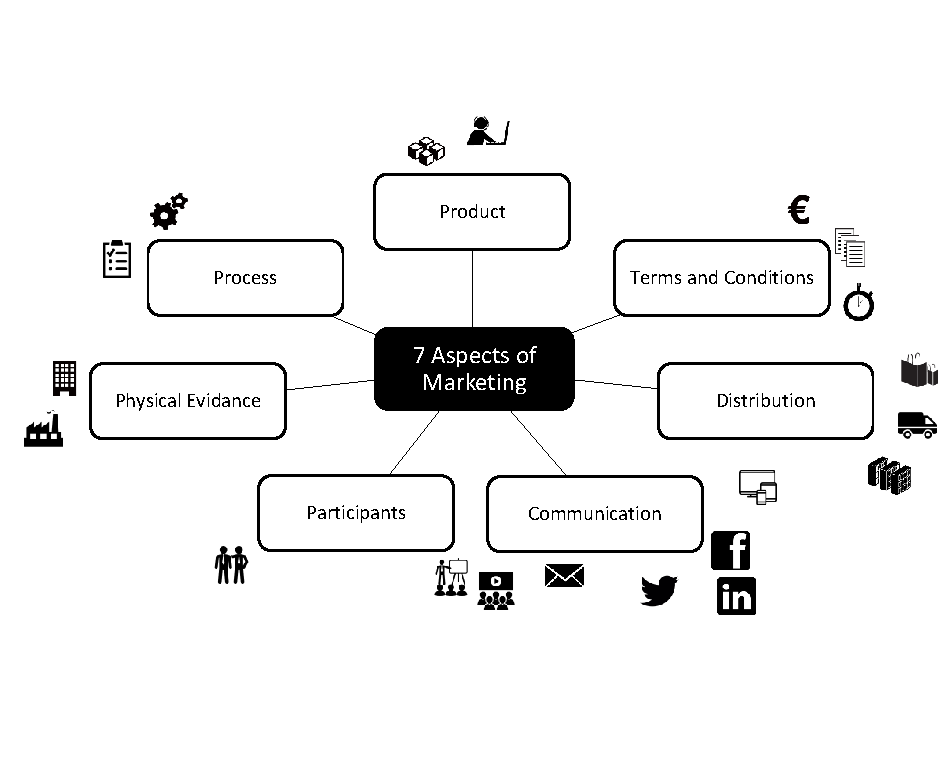
\includegraphics[width=\textwidth]{img/7p.pdf}
	\caption[Seven Aspects of Marketing]{The seven Aspects of Marketing as used in this paper (own illustration based on \protect\cites[285]{Thommen.2012}[397-720]{Meffert.2015}{Hoepner2015})}
	\label{fig:aspects}
\end{figure}

\begin{enumerate}
    \item{Product:}\\
    The value of the individual product to be sold alone, and as part of the program of the selling company \parencite[cf.][398]{Meffert.2015}. As an example, the iPhone has certain features. Additionally, it is part of the Apple's linecard, among the iPad, several Mac products and other things, including accessories and more. The individual product and its integration into the providers program can generate value to the customer, and different competitive advantages.
    
    \item{Terms and Conditions:}\\
    The terms and condition range from the price for purchase to service level agreements and warranty agreements, governing law, and many more \parencite{Hoepner2015}. As an example, it is possible for several software products to be purchased with drastically different service levels tied to different prices. 
    
    \item{Distribution:}\\
    The question of where and how you can purchase the product \parencite{Hoepner2015}. For instance, it is possible to purchase the iPhone in a wide variety of stores, including Apple Stores, online and at most mobile service providers. On the other hand, the first One Plus was only available online and only by being invited by someone legitimate.
    
    \item{Communication:}\\
    This includes for example commercials, public relations, as well as sales men \parencite{Hoepner2015}.
    
    \item{Participants:}\\
    The concrete individuals involved in placing the goods at the disposal. This includes for instance their skills and appearance. Someone dressed in a suit, may not be perceived as a creditable plumber\parencite{Hoepner2015}. 
    
    \item{Physical Evidence:}\\
    \textcite[155]{AzilaGbettor2013} cite \textcite{Booms.1981} as describing the physical evidence, the physical environment surrounding the service. This explicitly targets the premises and related entities \parencite[cf.]{Hoepner2015}.
    
    \item{Process Parts:}\\
    The process parts describe the process of the contract fulfillment \parencite{Hoepner2015}.
\end{enumerate}


\subsection{B2B versus B2C Marketing}

Several applications of the marketing instruments mentioned above are known from consumer market companies. Common examples are PayPal's Terms and Conditions containing their customer protection \parencite[see][]{PayPal} and the communication techniques of Apple. \textcite[20-21]{Backhaus.2015b} states that consumer marketing and industrial marketing differ in several points.


\begin{table}[H]
\begin{center}
\begin{tabular}{|c|c|c|}
\hline 
 & Industrial Marketing & Consumer Marketing \\ 
\hline 
Demand & Derived & Direct \\ 
\hline 
Customers & Organizations & People \\ 
\hline 
Decision makers & Mainly multiple people & Mainly sole people \\ 
\hline 
Requirements & Formalized & Not formalized \\ 
\hline 
Market & Identified & Anonymous \\ 
\hline 
\end{tabular} 
\end{center}
\caption[Differences between industrial and consumer marketing]{Differences between industrial and consumer marketing (own illustration based on \protect\cite[21]{Backhaus.2015b})}
\label{tab:marketingdiff}
\end{table}


As can be seen in \Cref{tab:marketingdiff}, the circumstances for industrial - or B2B - marketing differ. It is worth taking a note, which points influence the conception of a marketing application as it is desired by this paper. 

\paragraph*{Demand:} 
The demand of a consumer market is by definition direct demand, since it is caused by a consumer wanting or needing something. The suppliers for the requested goods themselves require goods and services in order to fulfill the consumer needs. Therefore the B2B demand is derived from the direct demand \parencite[cf.][21]{Backhaus.2015b}. This implies, that one marketing strategy must be planned in respect to the downstream demand down to the consumer. 

\paragraph*{Customers:} 
Because organizations - not people - are the target customers in B2B marketing, the legal and organizational complexity must be considered \parencite[cf.][21]{Backhaus.2015b}, as explained in the following two points.

\paragraph*{Decision makers:} 
Regarding consumer purchases, the dominant part is decided on by an individual. Organizations on the other hand have larger groups of people involved in such a decision \parencite[cf.][21]{Backhaus.2015b}. This results in not only more people that have to be convinced, but also in differing target groups for the same product, e.g. the financial department, the technical department, and some operating department. 

\paragraph*{Requirements:} 
In consumer markets, suppliers try to anticipate the needs of the customers, and offer goods and services designed by these assumptions. In the B2B market this is still true for some products, but in the specific field of this paper, customer companies define their requirements in their request for proposal \parencite[cf.][22]{Backhaus.2015b}. Therefore, it is possible to adapt the marketing mix to individual cases.